\begin{figure}[H]
	\centering
	\begin{tikzpicture}[node distance=1.5cm and 1cm, auto]
			% Nodo per immagine 3 con didascalia sotto, posizionato sotto img2
		\node (img1){
			\begin{tabular}{c}
				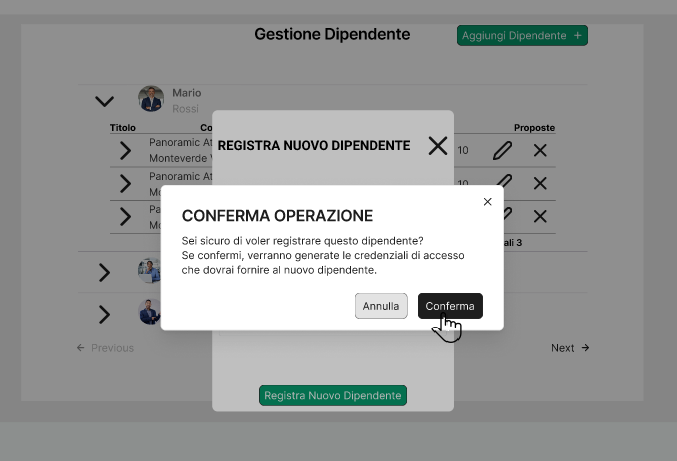
\includegraphics[width=0.7\textwidth]{Immagini/Mockup/nuovoAgente/scenario principale/ClickAllertConferma.png} \\
				Cockburn: step 6.D
			\end{tabular}
		};
		
		% Nodo per immagine 1 con didascalia sotto
		\node (img2)  [below=of img1] {
			\begin{tabular}{c}
				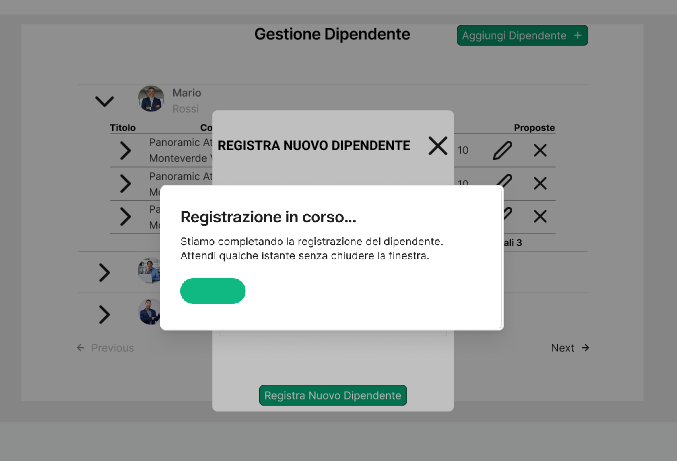
\includegraphics[width=0.7\textwidth]{Immagini/Mockup/nuovoAgente/scenario principale/caricamentoRegistrazione.png} \\
				Cockburn: step 7.D
			\end{tabular}
		};
		
		% Nodo per immagine 3 con didascalia sotto, posizionato sotto img2
		\node (img3) [below=of img2] {
			\begin{tabular}{c}
				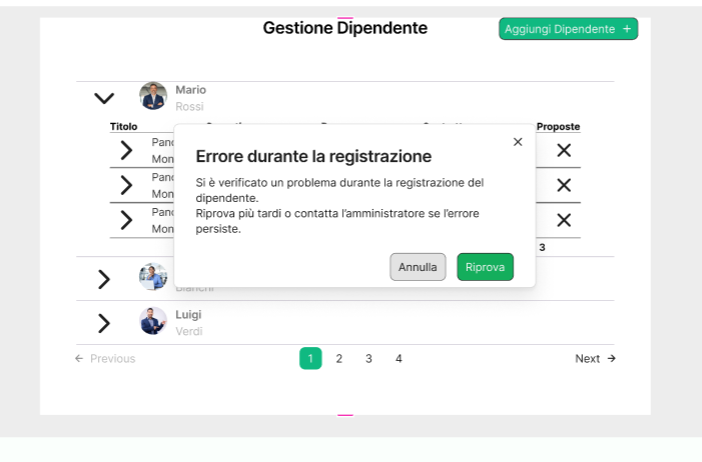
\includegraphics[width=0.7\textwidth]{Immagini/Mockup/nuovoAgente/extension D/messaggioDiErrore.png} \\
				Cockburn: step 8.D
			\end{tabular}
		};
		
		% Disegna le frecce
		\draw[->, thick] (img1) -- (img2);
		\draw[->, thick] (img2) -- (img3);
		
	\end{tikzpicture}
	\caption{Mockup: Extension D della tabella di Cockburn del caso d'uso: Registra nuovo agente.}
	\label{fig:tikz_flow}
\end{figure}